\documentclass[brazilian, fleqn]{article}

\usepackage{babel}
\usepackage[utf8]{inputenc}
\usepackage[T1]{fontenc}
\usepackage{lmodern}

\usepackage{amssymb,amsfonts,amsmath}

\DeclareMathOperator{\sen}{sen}

\usepackage[left=2cm, bottom=2cm, right=1.5cm, top=1.5cm]{geometry}

\usepackage{tikz}
\usetikzlibrary{decorations.pathmorphing,calc}
\tikzset{snake it/.style={decorate, decoration=snake}}

\usepackage{siunitx}
\sisetup{locale = FR}

\begin{document}

\section{Resolução do exemplo}
\begin{center}
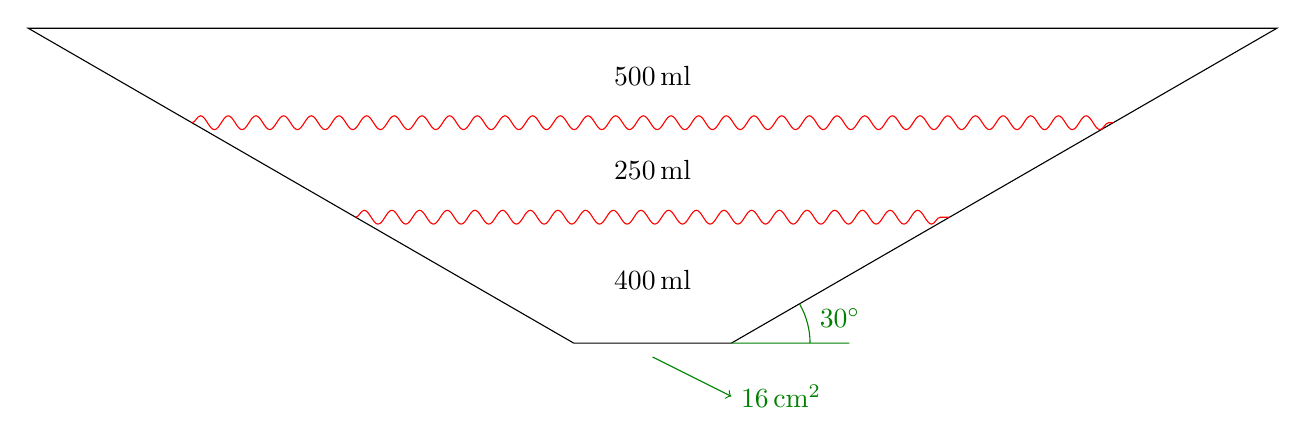
\begin{tikzpicture}[scale=1/2]
    \pgfmathsetmacro{\altura}{8}
    \draw (0,\altura) coordinate (A) --
        ({\altura/tan(30)},0) coordinate (B) -- 
        ++(4,0) coordinate (C) -- 
        ++({\altura/tan(30)},\altura) coordinate (D) -- cycle;
    \draw [red, snake it] ($(A)!0.3!(B)$) -- ($(D)!0.3!(C)$);
    \draw [red, snake it] ($(A)!0.6!(B)$) -- ($(D)!0.6!(C)$);
    \node at ($(B)!0.5!(C) + (0,{0.2*\altura})$) {\SI{400}{ml}};
    \node at ($(B)!0.5!(C) + (0,{0.55*\altura})$) {\SI{250}{ml}};
    \node at ($(B)!0.5!(C) + (0,{0.85*\altura})$) {\SI{500}{ml}};
    \draw [green!50!black] (C) -- +(0:2cm) node [above right, yshift=2pt] {\SI{30}{\degree}} arc (0:30:2cm) (C) -- +(0:3cm);
    \draw [green!50!black, ->] ([yshift=-1em] $(B)!0.5!(C)$) -- +(2cm,-1cm) node [right] {$\SI{16}{cm^2}$};
\end{tikzpicture}
\end{center}

\begin{itemize}
    \item Temos que o volume de um tronco de cone é dado por
        \[
            V=\frac{\pi h}{3} (R^2+Rr+r^2)
        \]
    \item \(\SI{16}{cm^2} \implies r_1 = \SI{2.26}{cm}\)
    \item \(R_1 = r_1 + h_1\tan{\SI{60}{\degree}}=r_1+\sqrt{3}h_1\)
    \item \(400 = \frac{\pi h_1}{3} ((r_1+\sqrt{3}h_1)^2+(r_1+\sqrt{3}h_1)r_1+r_1^2)\)
    \item \( r_1 = \SI{2.26}{cm} \implies h_1 = \SI{3.76}{cm} \implies R_1 = \SI{8.77}{cm}\)
    \item \( r_2 = \SI{8.77}{cm} \implies h_2 = \SI{0.87}{cm} \implies R_2 = \SI{10.28}{cm}\)
    \item \( r_3 = \SI{10.28}{cm} \implies h_3 = \SI{1.23}{cm} \)
    \item \(P_1 = P_2 + \rho_1 g h_1 = P_3+\rho_2 g h_2 + \rho_1 g h_1 = 0+\rho_3 g h_3 + \rho_2 g h_2 + \rho_1 g h_1\)
    \item \(F_1 = (\rho_1 h_1 + \rho_2 h_2 + \rho_3 h_3) A_1 g \)
\end{itemize}

\begin{center}
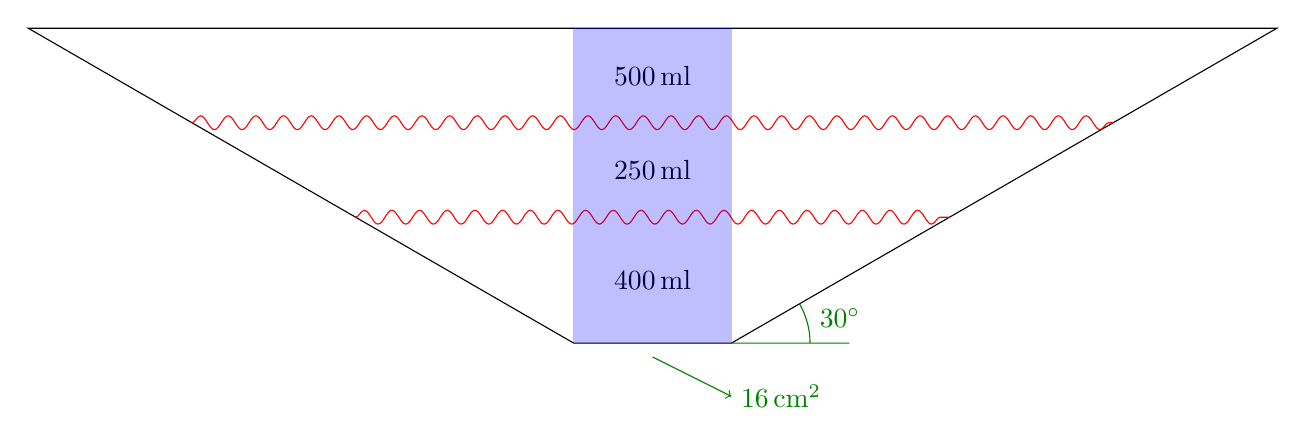
\begin{tikzpicture}[scale=1/2]
    \pgfmathsetmacro{\altura}{8}
    \draw (0,\altura) coordinate (A) --
        ({\altura/tan(30)},0) coordinate (B) -- 
        ++(4,0) coordinate (C) -- 
        ++({\altura/tan(30)},\altura) coordinate (D) -- cycle;
    \draw [red, snake it] ($(A)!0.3!(B)$) -- ($(D)!0.3!(C)$);
    \draw [red, snake it] ($(A)!0.6!(B)$) -- ($(D)!0.6!(C)$);
    \node at ($(B)!0.5!(C) + (0,{0.2*\altura})$) {\SI{400}{ml}};
    \node at ($(B)!0.5!(C) + (0,{0.55*\altura})$) {\SI{250}{ml}};
    \node at ($(B)!0.5!(C) + (0,{0.85*\altura})$) {\SI{500}{ml}};
    \draw [green!50!black] (C) -- +(0:2cm) node [above right, yshift=2pt] {\SI{30}{\degree}} arc (0:30:2cm) (C) -- +(0:3cm);
    \draw [green!50!black, ->] ([yshift=-1em] $(B)!0.5!(C)$) -- +(2cm,-1cm) node [right] {$\SI{16}{cm^2}$};
    \filldraw [blue, opacity=0.25] (B) rectangle ($(A)!(C)!(D)$);
\end{tikzpicture}
\end{center}
\end{document}
